\documentclass[a4paper]{article}
% mathmatical fonts and formulations
\usepackage{amsfonts}
\usepackage{amsmath}
\usepackage{amsthm}
\usepackage{amssymb}
% float control
\usepackage{placeins}
% graphic control
\usepackage{pgf}
\usepackage{tikz}
\usepackage{xcolor}
% excercise
%\usepackage{exercise}
% Algorithm support
%\usepackage{algorithmic}
\usepackage{algorithm2e}
% Set space
\usepackage[top=1.54cm,bottom=1.54cm,left=3.18cm,right=2.54cm,includehead,includefoot
           ]{geometry}
%color of the word
\usepackage{color}
% change the counter of enumerate
\usepackage{enumerate}
% allow to use the block
\usepackage{framed}
% introduce indent at the beginning of every pragraph
\usepackage{indentfirst}
% every section begins at a new page
%\usepackage{titlesec}
\newcommand{\sectionbreak}{\clearpage}

\theoremstyle{definition}
\newtheorem{lemma}{Lemma}[section]
\newtheorem{theorem}{Theorem}[section]
\newtheorem{definition}{Definition}[section]
\newtheorem{corollary}{Corollary}[section]
\newtheorem{exercise}{Exercise}[section]
\newtheorem{example}{Example}[section]
\newtheorem{observe}{Observation}[section]

\date{}
\author{}
\title{COMP3721 Tutorial 8}

% set the way to number equation
\numberwithin{equation}{subsection}
%depth of table of contents
\setcounter{tocdepth}{2}
\begin{document}
\maketitle
\section{Turing Machines}
\begin{enumerate}[Q1.]
\item Knowing that $M = (K,\Sigma, \delta, s, H)$, give the mathematical definition of the following Turing machine.
\begin{center}
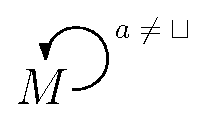
\includegraphics[scale = 0.6]{q1.eps}
\end{center} 

\item Explain what this machine does on the input $\triangleright\underline{\sqcup} w$.
\begin{center}
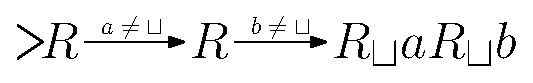
\includegraphics[scale = 0.6]{q2.eps}
\end{center} 

\item Trace the operation of the following Turing machine when started on $\triangleright{\sqcup} aabb\underline{\sqcup}$.
\begin{center}
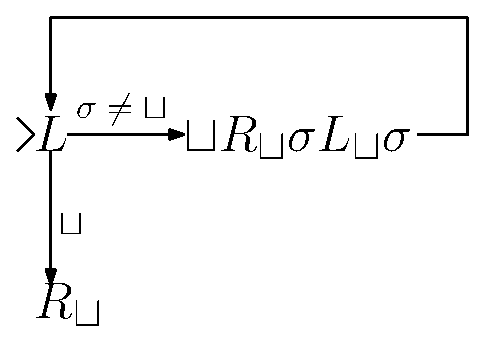
\includegraphics[scale = 0.6]{q3.eps}
\end{center}
\end{enumerate}
\end{document}

